\section{Dynamically condensed colour codes}\label{sec:dynamically-condensed-colour-codes}

As a first case study in dynamic stabilizer codes, we now look at \textit{dynamically condensed colour codes} (DCCCs).
As the name suggests, the starting point for these codes is the colour code, which we defined back in \Cref{ex:colour_code_stabilizer_code}.
Diagrams in this subsection should be read bottom-to-top, and we will employ our new ability to choose any representative of a diagram in the $\zxmodpi$-calculus, freely omitting `measurement spiders'.

\subsection{Bosons of the colour code}

DCCCs can be defined in terms of the colour code's \textit{boson table}; this name (and other terminology below) comes from a more condensed matter perspective on the colour code.
If the word boson means nothing to you, no problem -- it means nothing to me either!
All you need to know is that this boson table is a $3 \times 3$ grid with columns labelled by colours $\colourful{c}, \colourful{m}$ and $\colourful{y}$ (cyan, magenta, and yellow)
and rows labelled by letters $X, Y$ and $Z$ (non-identity Pauli matrices).
Cells of the table are thus colour-Pauli pairs $(\kappa, P)$.
Often we will want to talk about generic colours $\{\kappa, \kappa', \kappa''\} = \{\colourful{c}, \colourful{m}, \colourful{y}\}$
and generic Pauli matrices $\{P, P', P''\} = \{X, Y, Z\}$,
for which we will use a boson table with these generic labels instead:
\begin{equation}\label{eq:cc_boson_table}
\bosonTable{
    rx={\colourful{c}, X},
    gx={\colourful{m}, X},
    bx={\colourful{y}, X},
    ry={\colourful{c}, Y},
    gy={\colourful{m}, Y},
    by={\colourful{y}, Y},
    rz={\colourful{c}, Z},
    gz={\colourful{m}, Z},
    bz={\colourful{y}, Z},
}
\qquad \text{or} \qquad
\bosonTable{
    rx={\kappa, P},
    gx={\kappa', P},
    bx={\kappa'', P},
    ry={\kappa, P'},
    gy={\kappa', P'},
    by={\kappa'', P'},
    rz={\kappa, P''},
    gz={\kappa', P''},
    bz={\kappa'', P''},
}
\end{equation}

Just like the colour code, a DCCC can be defined on any three-face-colourable, three-valent planar graph,
and edges in such a graph inherit a canonical coluuring from the faces.
Throughout this chapter we use the honeycomb lattice.
We also assume throughout that this lattice is placed on a torus.

Recall when we introduced the colour code we defined edge and face operators;
for every cell $(\kappa, P)$ of the boson table, we get a \textit{$(\kappa, P)$ edge operator} $\dcccOp{e}{\kappa}{P} \coloneqq P_{v_0} P_{v_1}$ for every $\kappa$-coloured edge $e_\kappa = (v_0, v_1)$, and a \textit{$(\kappa, P)$ face operator} $\dcccOp{f}{\kappa}{P} \coloneqq P_{v_0} P_{v_1} \ldots P_{v_5}$ for every $\kappa$-coloured face $f_\kappa$ with vertices $v_0, v_1, \ldots, v_5$.
We define the set of all $(\kappa, P)$ edge operators as $\dcccOp{E}{\kappa}{P}$ and the set of all $(\kappa, P)$ face operators as $\dcccOp{F}{\kappa}{P}$.
Note that each face operator $\dcccOp{f}{\kappa}{P}$ can be made from edge operators in two ways; as the product of the three $(\kappa', P)$ edge operators around $f$, or the three $(\kappa'', P)$ edge operators.
Additionally, it can be written as the product of the other two face operators $\dcccOp{f}{\kappa}{P'}$ and $\dcccOp{f}{\kappa}{P''}$ on $f$, up to global phase.
Examples of such operators are shown in \Cref{fig:edge_and_face_operator}.

\begin{figure}[tbp]
    \centering
    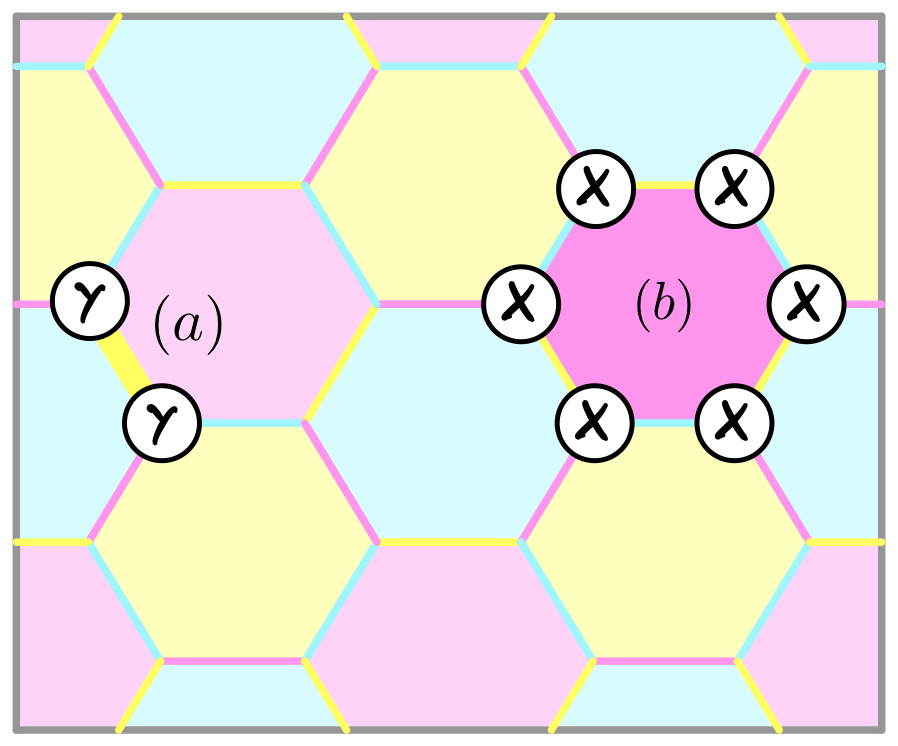
\includegraphics[width=180pt]{figures/qubits/dcccs/prelims/edge_and_face_operator}
    \caption{
        $(a)$ A $Y^{\otimes 2}$ yellow edge operator $e_{\textcolor{Dandelion}{y}, {Y}}$.
        $(b)$ An $X^{\otimes 6}$ magenta face operator $f_{\textcolor{magenta}{m}, {X}}$.
    }
    \label{fig:edge_and_face_operator}
\end{figure}

\subsection{Operation schedule}\label{subsec:measurement_schedule}

\begin{figure}[tbp]
    \centering
    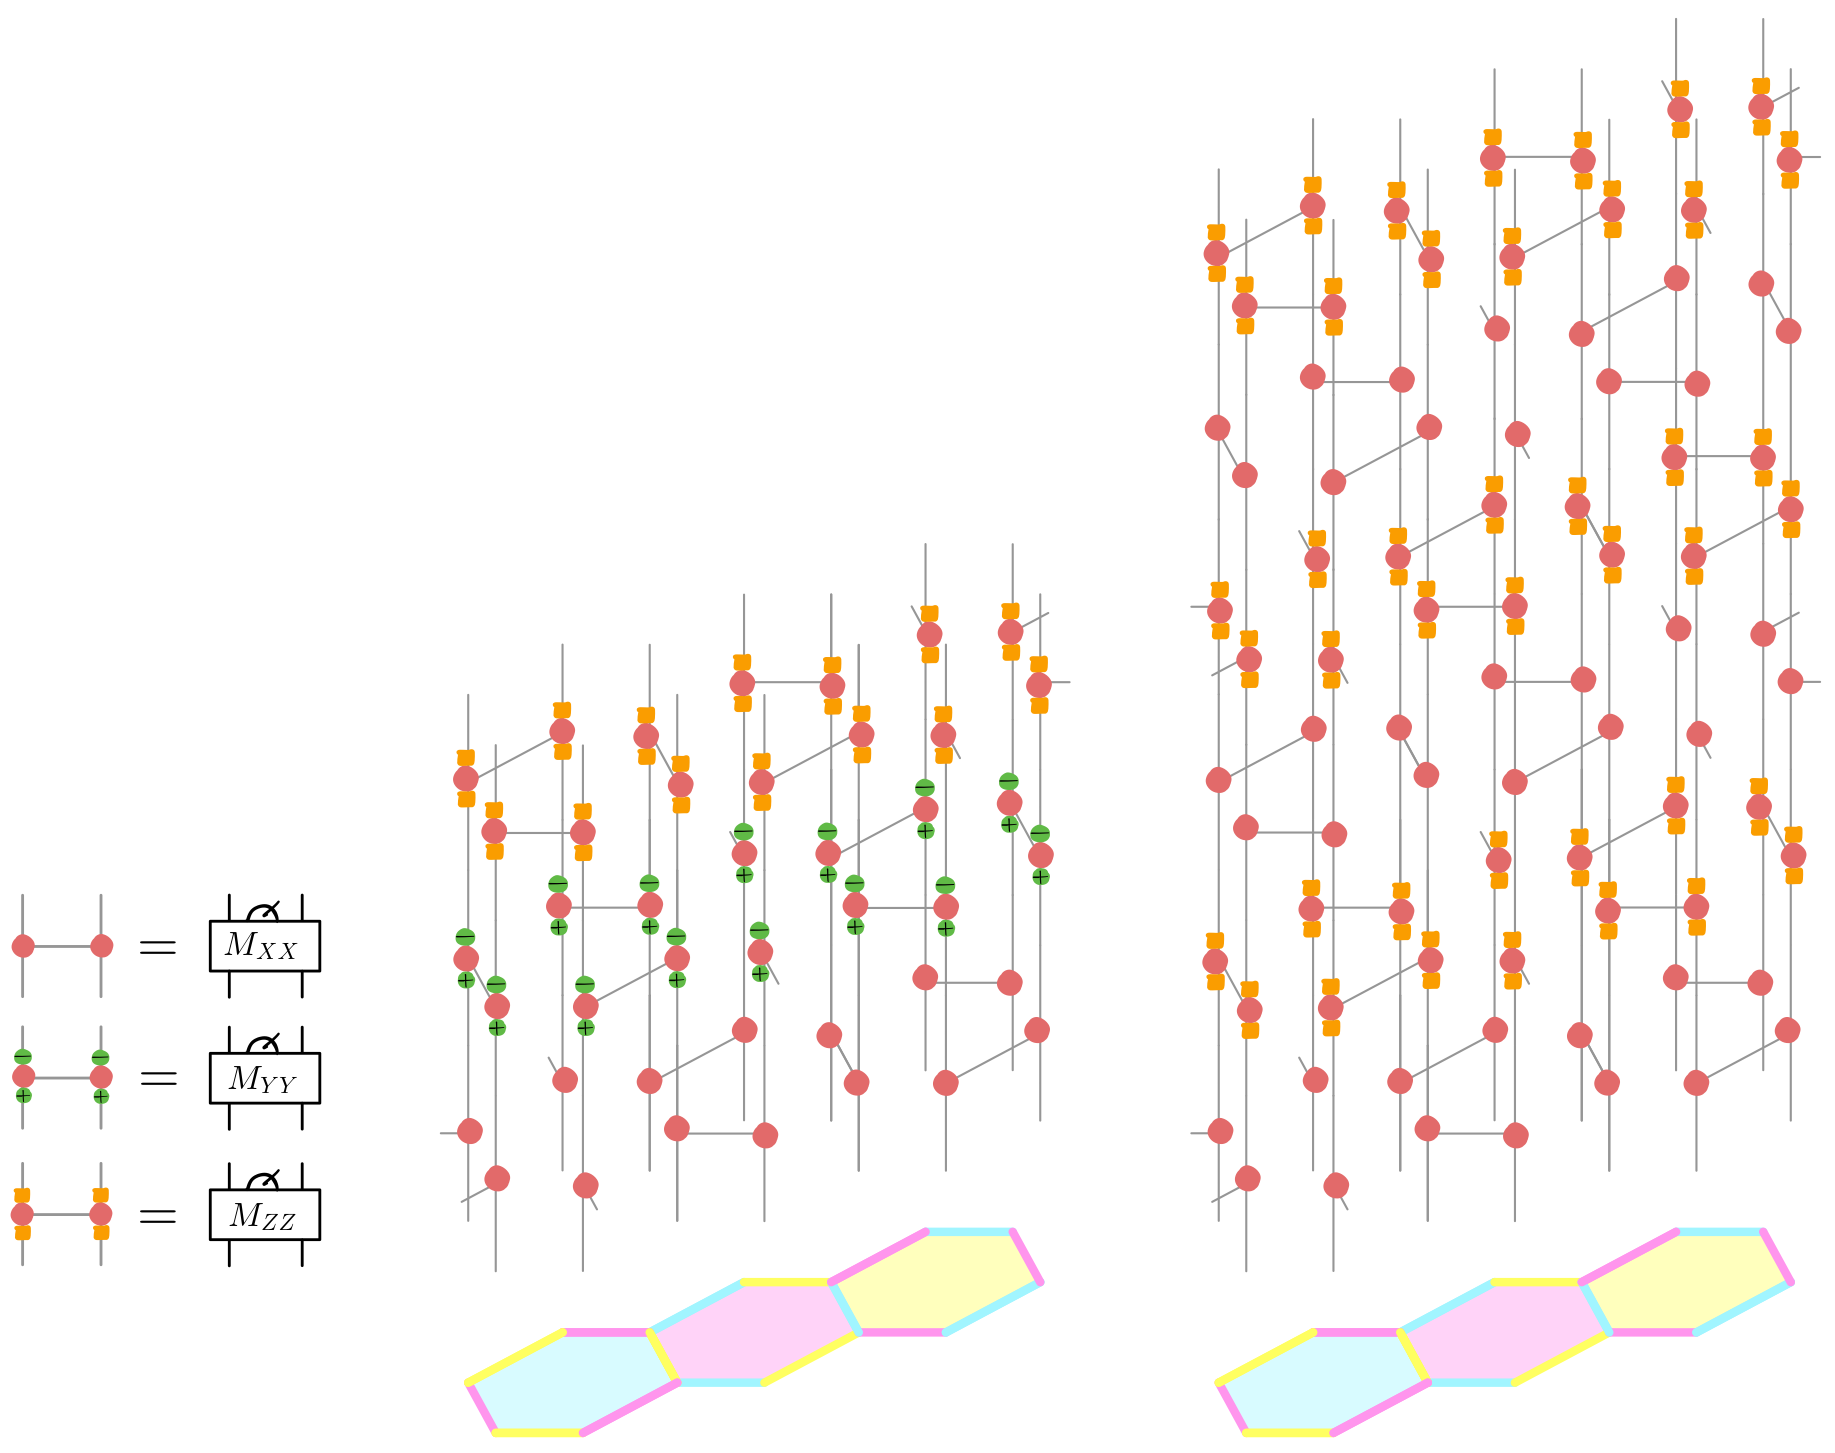
\includegraphics[width=\linewidth]{figures/qubits/dcccs/prelims/schedules_XYZ_and_CSS_measurements_next_to}
    \caption{
        For a subset of qubits, we show the sequence of measurements defining the $X^1 Y^1 Z^1$ (middle) and $X^1 Z^1$ (right) honeycomb codes.
        \teague{TODO remove measurement equalities on left.}
    }
    \label{fig:schedules_XYZ_and_CSS}
\end{figure}

A DCCC, then, is a dynamic stabilizer code defined by
repeatedly measuring sets $\dcccOp{E}{\kappa}{P}$ of all $(\kappa, P)$ edge operators.
That is, abusing notation again by just writing the Pauli $P$ to be measured rather than the operation $M_P$, it has operation sequence $\left(\dcccOp{E}{\kappa_0}{P_0},\dcccOp{E}{\kappa_1}{P_1},\ldots\right)$.
(Note the contrast to the colour code, where we measure face operators.)
For DCCCs as defined in \Ccite[Section 7]{kesselring2022anyon}, there is a single restriction:
if at time $t$ the operators $\dcccOp{E}{\kappa_t}{P_{t}}$ are measured,
then at time $t+1$ we must choose a new set $\dcccOp{E}{\kappa_{t+1}}{P_{t+1}}$ of edges to measure,
such that cell $(\kappa_{t+1}, P_{t+1})$ shares neither a row nor column with $(\kappa_t, P_t)$ in the boson table.
For reasons that will become clear shortly, we call DCCCs defined according to this rule `unrepeated' DCCCs.
The two unrepeated DCCCs we will focus on are
the \textit{$X^1Y^1Z^1$ honeycomb code} and the \textit{$X^1Z^1$ honeycomb code}.
These are defined by the operation sequences:
\begin{equation}\label{eq:honeycomb_codes_measurement_schedules}
\begin{aligned}
    \OOO_{X^1Y^1Z^1} &= \left(
    \dcccOp{E}{c}{X},
    \dcccOp{E}{m}{Y},
    \dcccOp{E}{y}{Z}
    \right)\\
    \OOO_{X^1Z^1} &= \left(
    \dcccOp{E}{c}{X},
    \dcccOp{E}{m}{Z},
    \dcccOp{E}{y}{X},
    \dcccOp{E}{c}{Z},
    \dcccOp{E}{m}{X},
    \dcccOp{E}{y}{Z}
    \right)
\end{aligned}
\end{equation}

\subsection{Establishment and logical Pauli group}

Every DCCC on a torus encodes $k=2$ logical qubits after establishment at time $T$.
(Again, note the contrast to the colour code on a torus, which encodes $4$ logical qubits.\footnote{This is because condensing the colour code essentially turns it into the surface code. A condensed matter theorist would be able to tell you more about this -- I cannot!})
Alternatively, we can always just ignore one of the logical qubits and pretend it only encodes one qubit; this makes our work more straightforward to compare with the more easily implementable planar case, which encodes just one logical qubit, and allows us to tailor the code dimensions to biased noise models later on.
In the rest of this section, we will do exactly this.
In \Cref{fig:logicals_XYZ_and_XZ}, we show representatives of logical $X$ and $Z$ operators for the $X^1Y^1Z^1$ and $X^1Z^1$ honeycomb codes at timesteps $t$ mod $6$.
Sticking with the condensed matter terminology, we will actually call these $E$ and $M$ logical operators rather than $X$ and $Z$.

\begin{figure}[tbp]
    \centering
    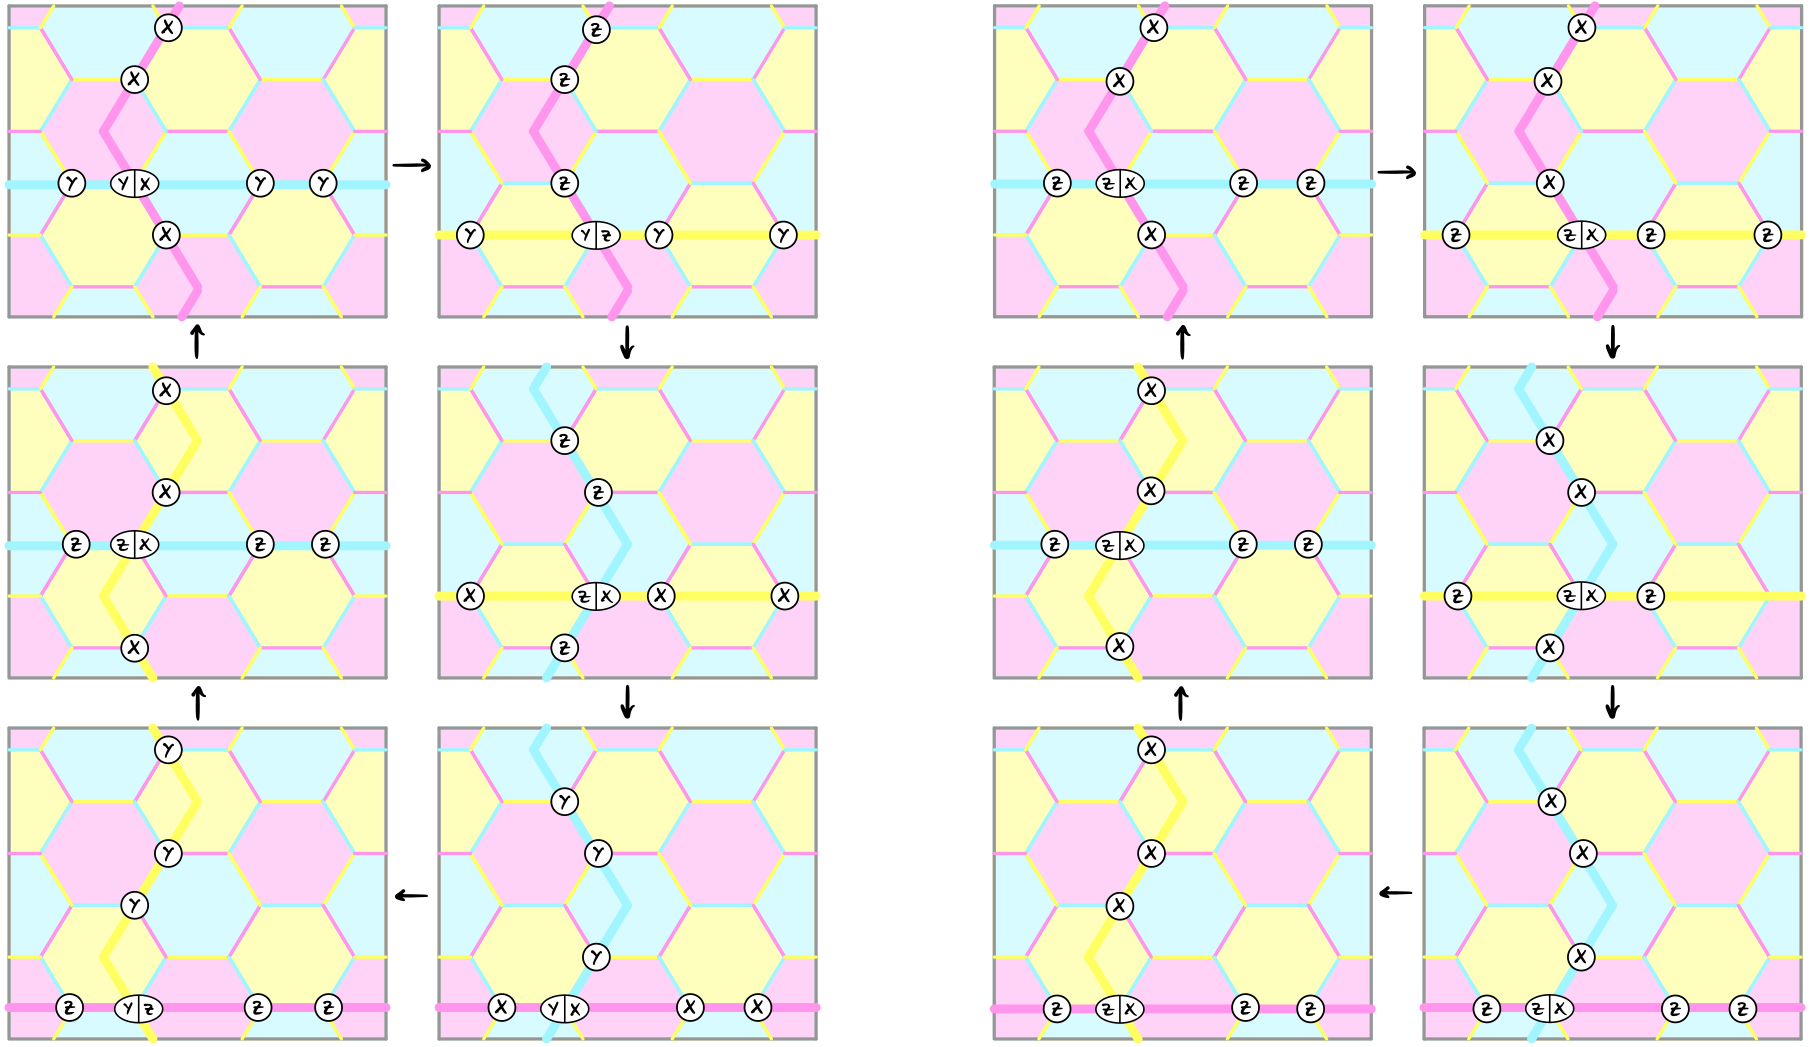
\includegraphics[width=\linewidth]{figures/qubits/dcccs/prelims/logicals_XYZ_and_XZ_stacked_horizontal}
    \caption{
        Representatives of logical $E$ and $M$ operators for the $X^1 Y^1 Z^1$ (left) and $X^1 Z^1$ (right) honeycomb codes at timesteps $t$ mod $6$.
        Timestep $0$ mod $6$ is the top left subfigure in each cycle.
        Boundaries are periodic, forming a torus.
        Throughout this section we say a DCCC encodes only one logical qubit - we just ignore the other one.
        We arbitrarily choose that the $E$ logical operator wraps vertically around the torus in this figure, with the $M$ operator wrapping around horizontally.
        Importantly, the representative of the $E$ operator in the $X^1 Z^1$ code always consists of Pauli $Z$ operators, and the $M$ operator always consists of Pauli $X$ operators.
        In the $X^1 Y^1 Z^1$ code, in contrast, the representatives of both the $E$ and $M$ operator consist one third of the time of Pauli $X$ operators, one third of the time of $Y$ operators and one third of the time of $Z$ operators.
        This will be important when discussing the effects of biased noise later on.}
    \label{fig:logicals_XYZ_and_XZ}
\end{figure}

\subsection{Detectors}

We let $m_t(\dcccOp{e}{\kappa_t}{P_t})$ denote
the outcome of measuring the edge operator $\dcccOp{e}{\kappa_t}{P_t}$ at time $t$,
and let $e \in f$ mean edge $e$ borders face $f$.
DCCCs have detectors\footnote{%
    This statement only holds if we make a distinction between detectors and \textit{observables}.
    An observable here doesn't have the usual meaning of a self-adjoint operator.
    Instead it refers to a special detector that's used to test whether the decoder correctly decoded the errors in a circuit~\cite{Gidney2021stimfaststabilizer,derks2024}.
    There are indeed observables that are not of this form.}
of the form $d = \prod_{t \in \tau} \prod_{e_{\kappa_t} \in f_{\kappa}} m_t(\dcccOp{e}{\kappa_t}{P_t})$
for some set of timesteps $\tau$ and some $\kappa$-coloured face $f_\kappa$.
For example, on the left of \Cref{fig:detectors_XYZ_and_CSS} we show a detector in the $XYZ$ honeycomb code,
and on the right a detector in the CSS honeycomb code,
both associated to some yellow face $f_{\colourful{y}}$.
As a formal product, with timesteps taken modulo 6, the former is written as:
\begin{equation}\label{eq:XYZ_detector_yellow}
\prod_{e_{\colourful{m}} \in f_{\colourful{y}}} m_4(\dcccOp{e}{m}{Y})
\prod_{e_{\colourful{c}} \in f_{\colourful{y}}} m_3(\dcccOp{e}{c}{X})
\prod_{e_{\colourful{m}} \in f_{\colourful{y}}} m_1(\dcccOp{e}{m}{Y})
\prod_{e_{\colourful{c}} \in f_{\colourful{y}}} m_0(\dcccOp{e}{c}{X})
\end{equation}
while the latter is:
\begin{equation}\label{eq:CSS_detector_yellow}
\prod_{e_{\colourful{m}} \in f_{\colourful{y}}} m_4(\dcccOp{e}{m}{X})
\prod_{e_{\colourful{c}} \in f_{\colourful{y}}} m_0(\dcccOp{e}{c}{X})
\end{equation}

\begin{figure}[btp]
    \centering
    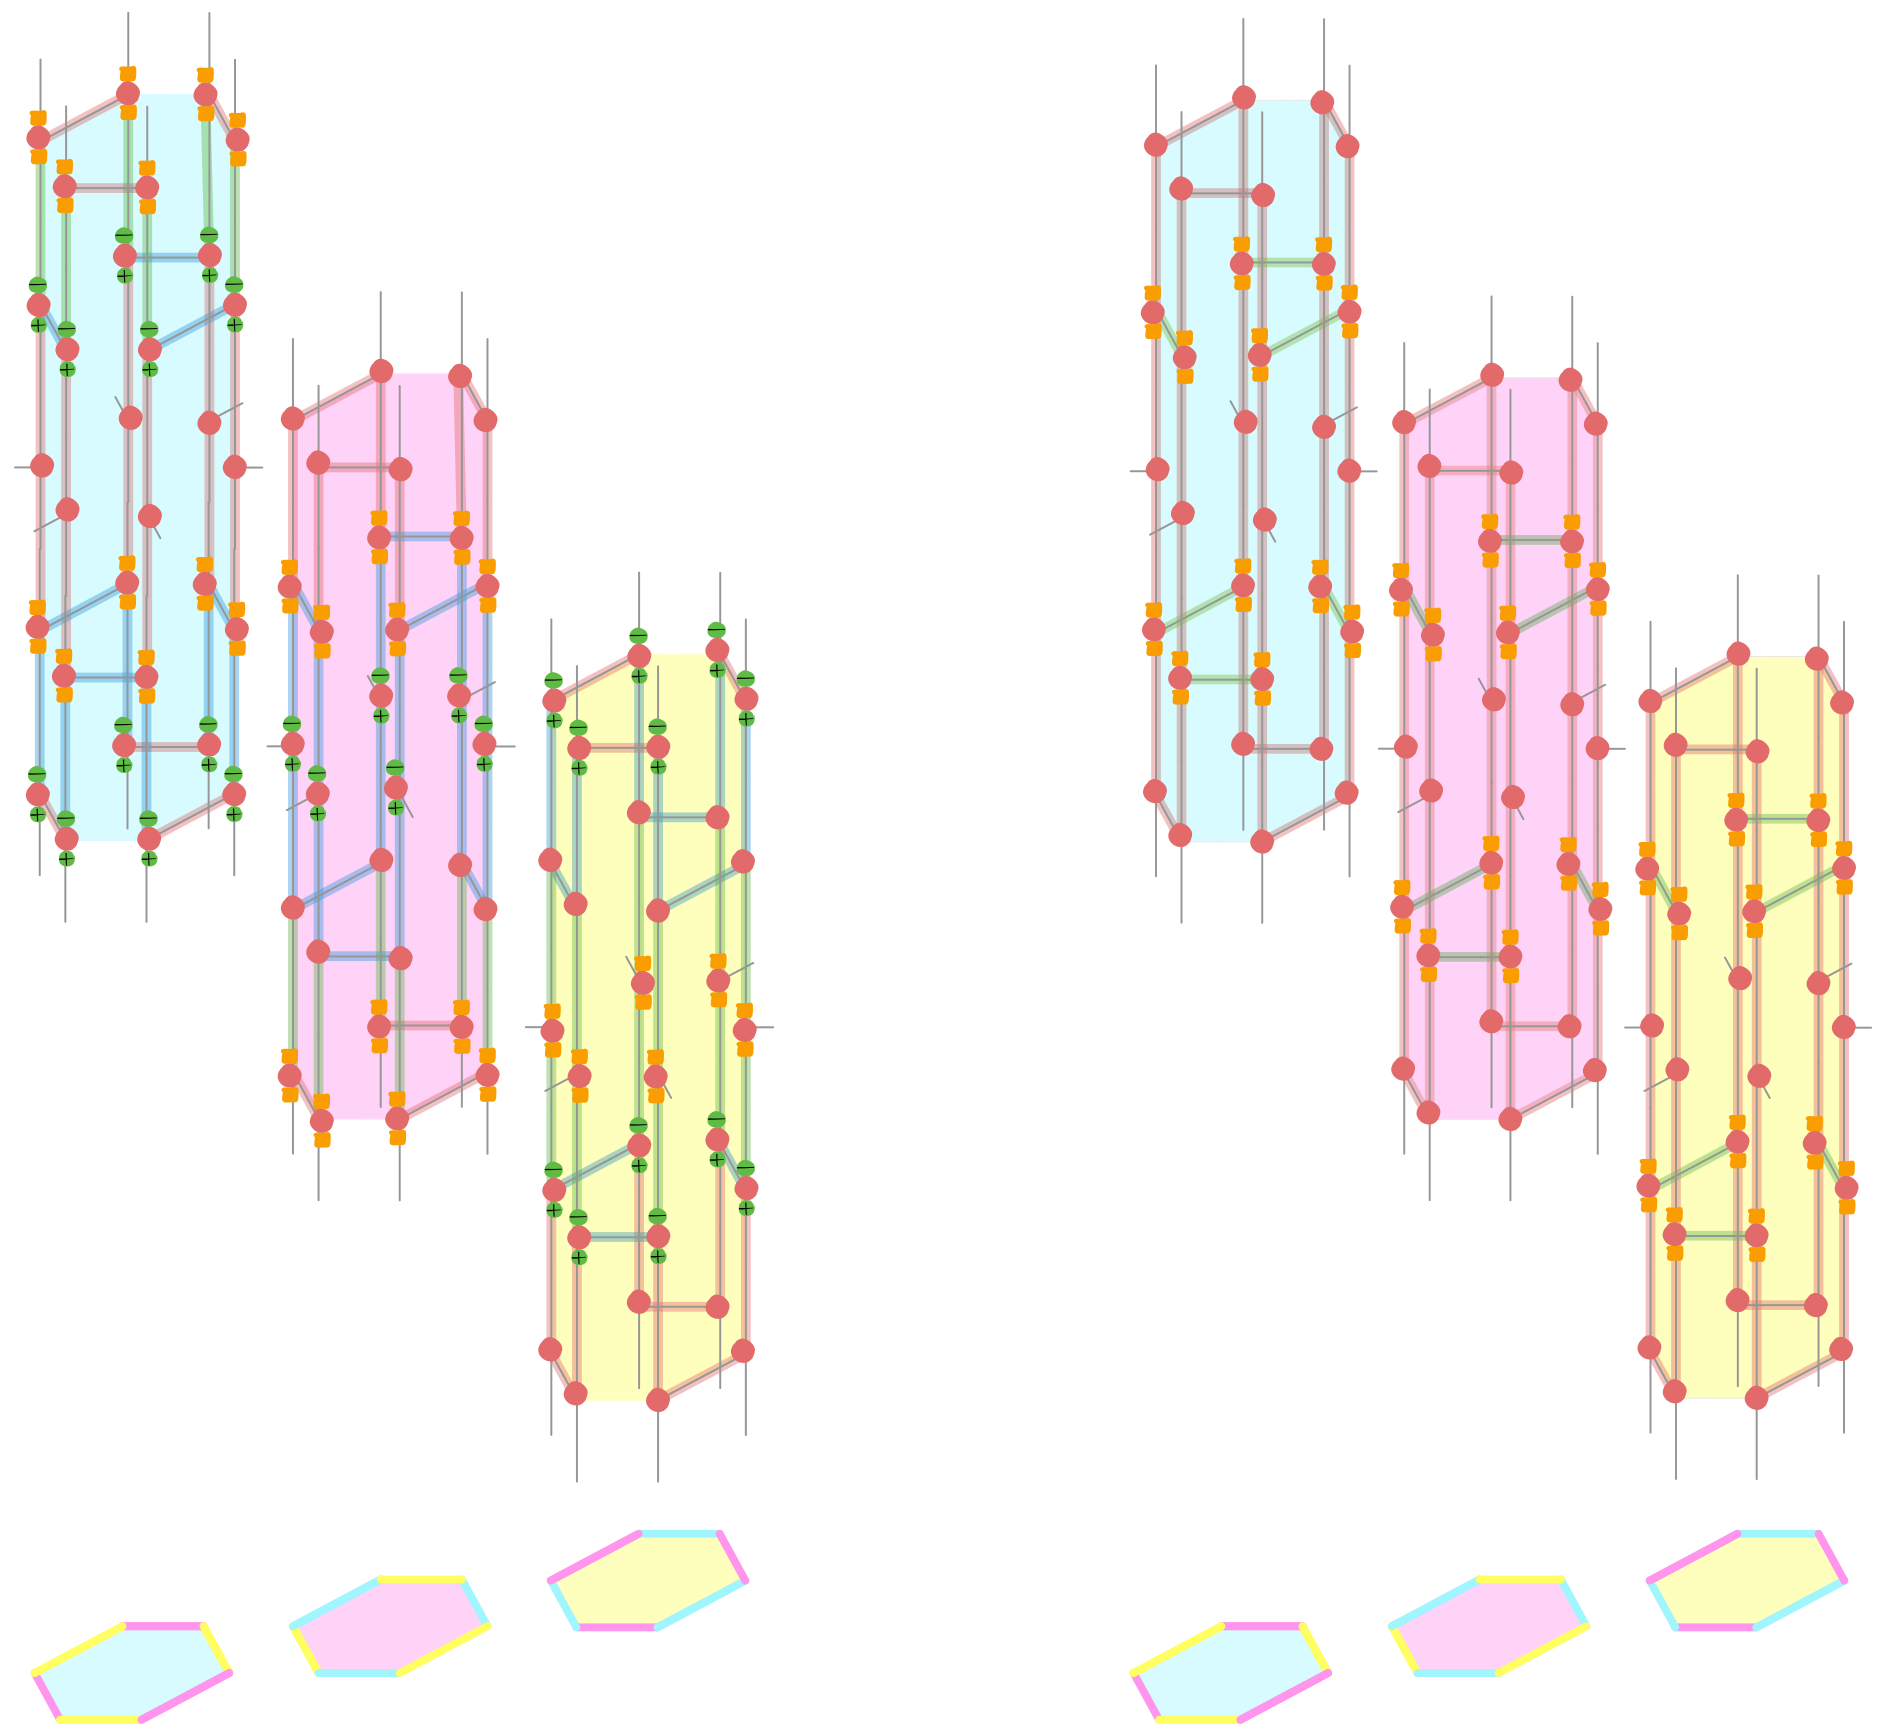
\includegraphics[width=\linewidth]{figures/qubits/dcccs/prelims/detectors_XYZ_and_CSS}
    \caption{
        A subset of detectors of the $X^1 Y^1 Z^1$ code (left) and the $X^1 Z^1$ code (right).
        A detector is violated by a set of errors if there's an odd number of them of a different colour to the highlighted wire they sit on (\Cref{cor:firing-detector-web-exact-scalar}).
        Pauli webs also tell us which measurements are actually involved in a detector and which are not; it's all mesurements corresponding to non-vertical edges highlighted red or blue.
    }
    \label{fig:detectors_XYZ_and_CSS}
\end{figure}

%\subsection{Logical errors}
%
%Recall TODO that logical errors are those that are undetectable but non-trivial.
%In a DCCC, we can further label logical errors as \textit{spacelike} or \textit{timelike}.
%Intuitively, spacelike logical errors are those consisting of sets of errors wrapping around the torus on which the code is defined (in either direction), and timelike logical errors are those consisting of sets of errors that span from the start of the circuit to the end.
%(A more rigorous but still digestible definition of spacelike and timelike would probably have to start using some fancier language, like \textit{homology groups} of \textit{fault complexes}, so we won't give such a definition!).
%For example, if after some timestep $t$ a set of qubit errors occur whose tensor product is a logical Pauli operator for the code at this timestep $t$ -- like those depicted in \Cref{fig:logicals_XYZ_and_XZ} -- then this constitutes a spacelike logical error.
%In \Cref{fig:XYZ_logical_data_qubit_errors}, we show one spacelike and one timelike logical error in the $X^1Y^1Z^1$ honeycomb code.
%
%The notion of distance (TODO definition) therefore also can be split into \textit{spacelike distance} or \textit{timelike distance} -- the minimum number of errors (under a given error model) required to create a spacelike or timelike logical error, respectively.
%
%\begin{figure}[htbp]
%    \centering
%    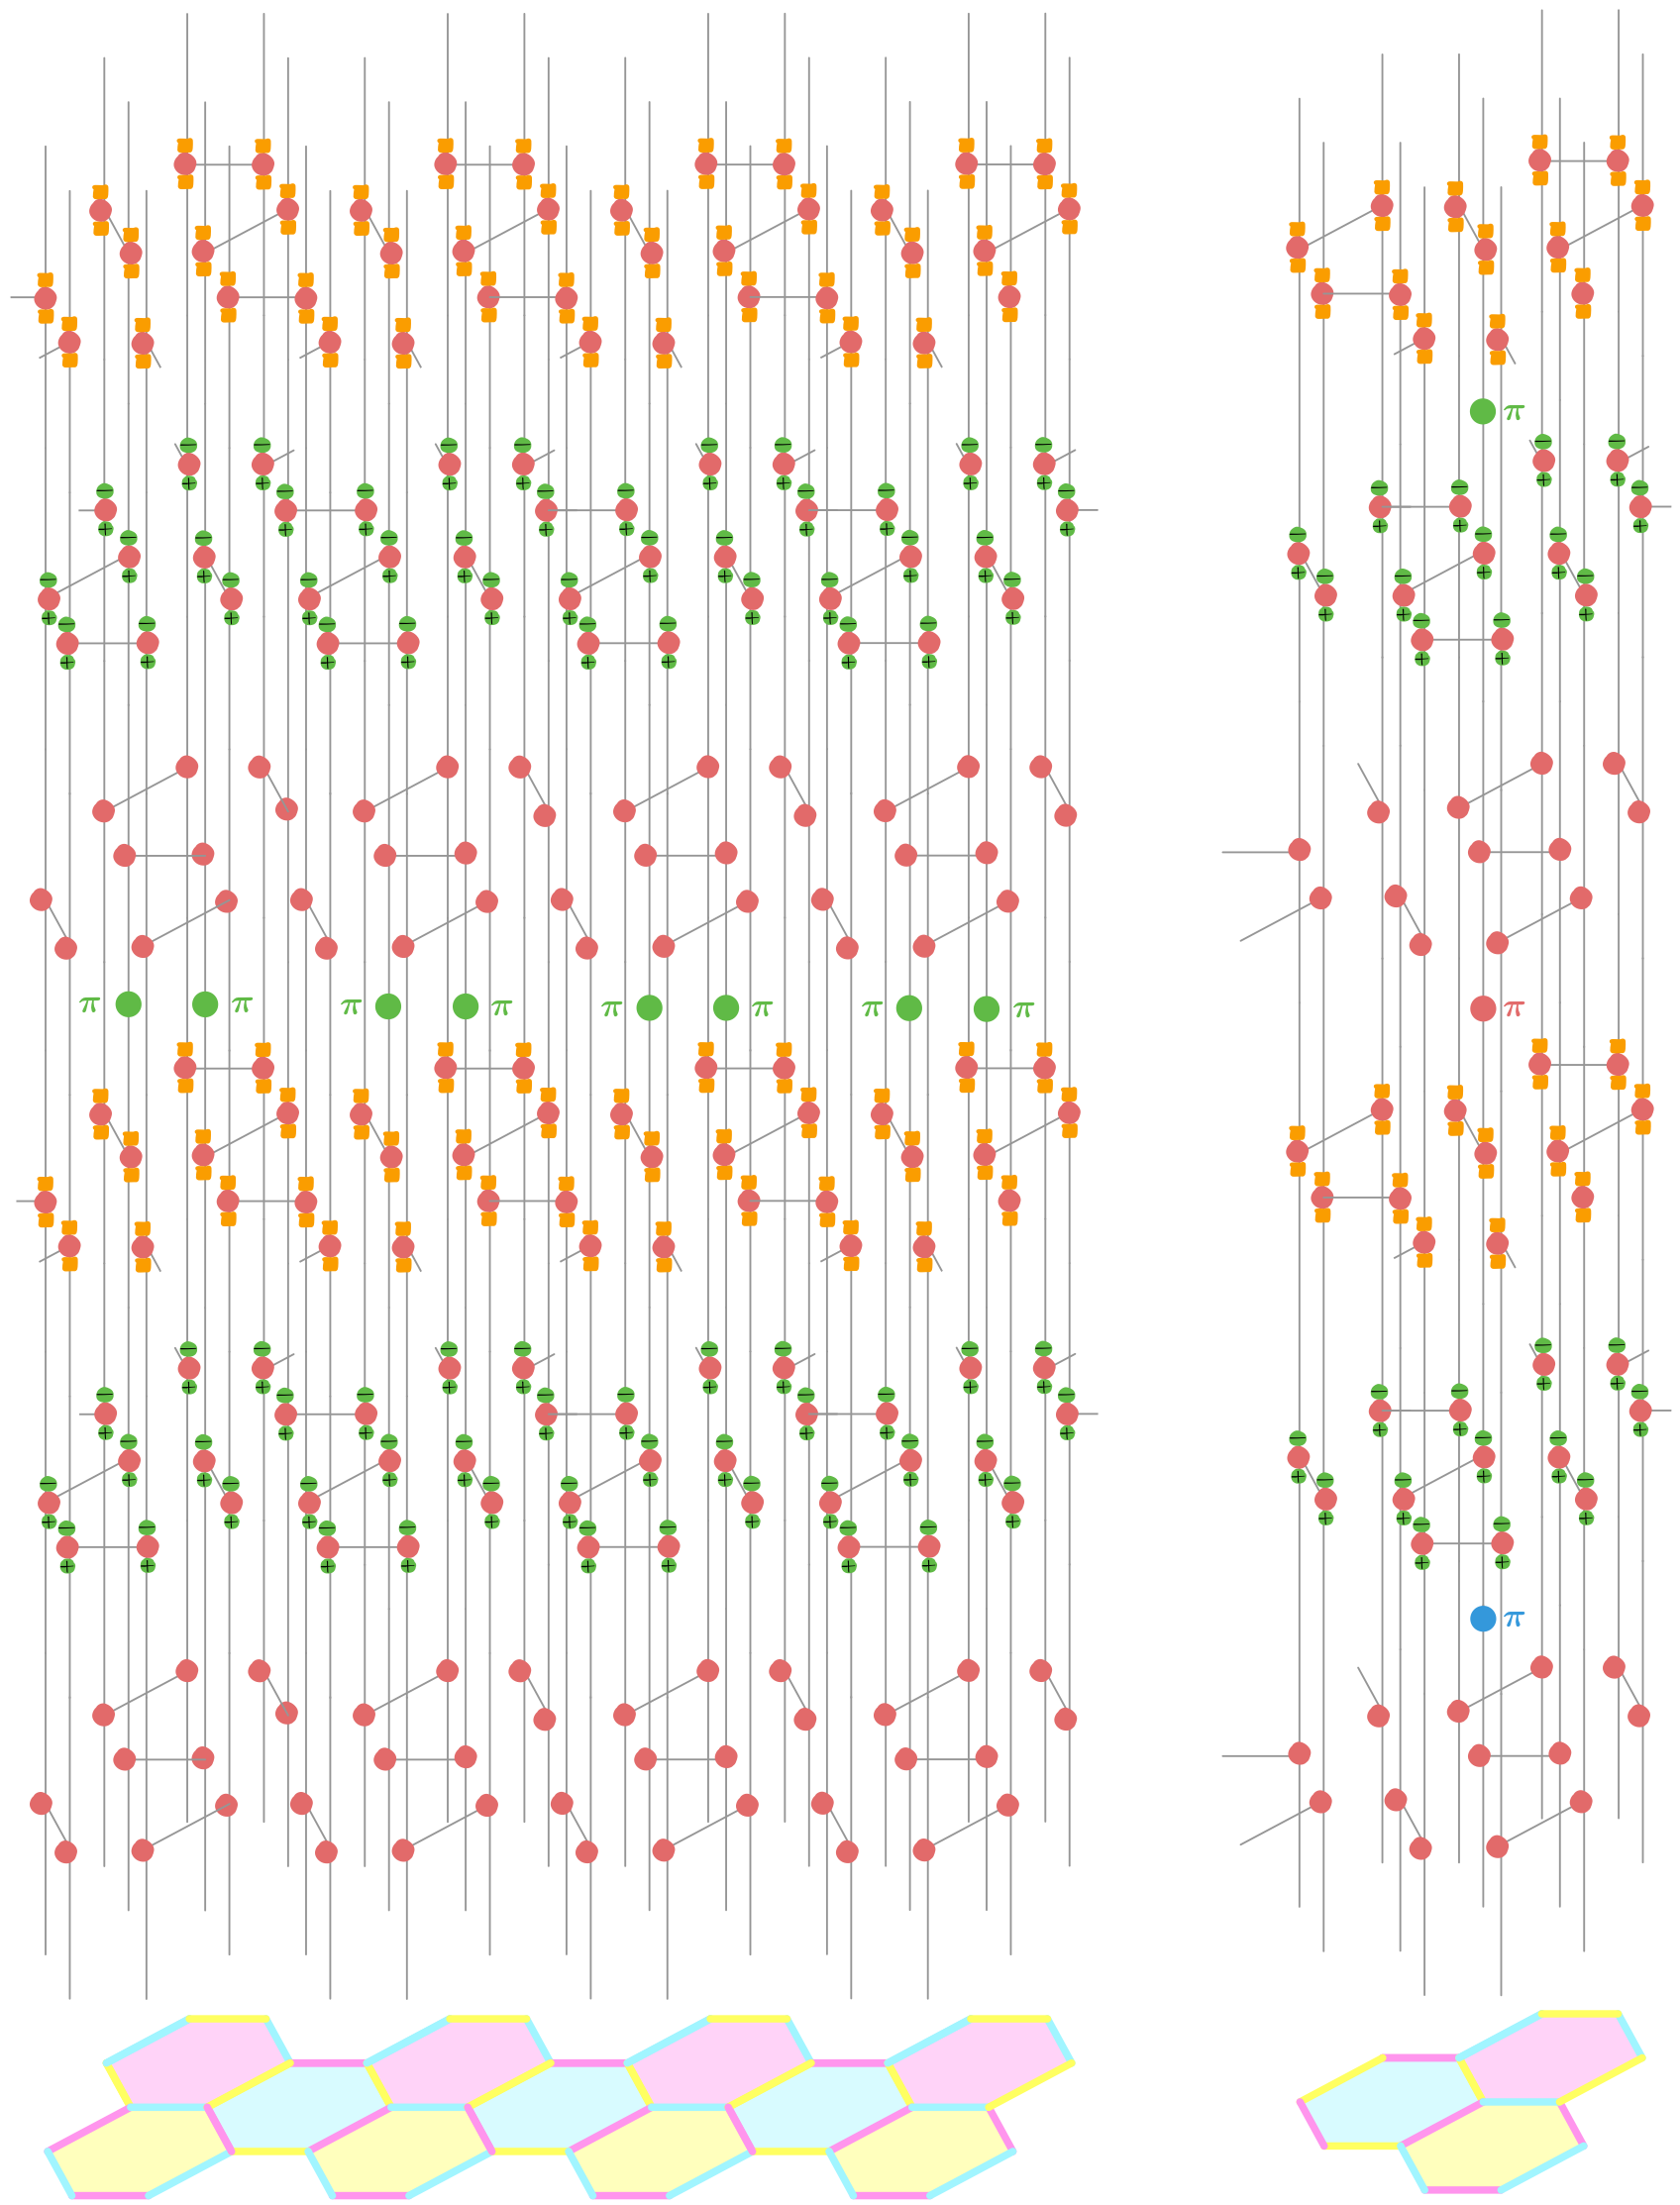
\includegraphics[width=\linewidth]{figures/qubits/dcccs/prelims/XYZ_logical_data_qubit_errors}
%    \caption{
%        On a subset of qubits, we show a spacelike (left) and timelike (right) logical error in the XYZ honeycomb code consisting only of data qubit errors.}
%    \label{fig:XYZ_logical_data_qubit_errors}
%\end{figure}

%\subsection{Bias-tailoring I: choosing a schedule}
%
%The choice of measurement schedule significantly impacts DCCC performance under different noise models.
%We first outline the major differences between the $X^1Y^1Z^1$ and $X^1Z^1$ honeycomb codes, and the expected effects on their performance.
%
%\begin{difference}\label{dif:XYZ_XZ_meas_per_detector}
%Detectors in the $X^1 Y^1 Z^1$ code consist of 12 measurements, while detectors in the $X^1 Z^1$ code consist of 6 measurements (\Cref{fig:detectors_XYZ_and_CSS}).
%\end{difference}
%
%Fewer measurements per detector generally improves performance, as the decoder has fewer violated detectors to handle.
%So this difference between the two codes would suggest the $X^1 Z^1$ code might generally perform better -- especially for measurement-biased noise.
%
%\begin{difference}\label{dif:XYZ_XZ_timelike_distance}
%The $X^1 Y^1 Z^1$ code implemented for $h$ rounds has a timelike distance of $h/2$, while the $X^1 Z^1$ code implemented for $h$ rounds has a timelike distance of $h/4$ (\Cref{tab:xyz_css_summary}, \Cref{fig:repeated_measurements_timelike_distances}).
%\end{difference}
%
%In contrast to \Cref{dif:XYZ_XZ_meas_per_detector} above, this difference favours the $X^1 Y^1 Z^1$ code;
%based on this alone, one would expect the $X^1 Y^1 Z^1$ code to perform better than the $X^1 Z^1$ code in \textit{stability experiments} (which examine the timelike distance of a code).
%
%\begin{difference}\label{dif:XYZ_XZ_hyperedges}
%All measurement errors in the $X^1 Y^1 Z^1$ code correspond to degree $> 2$ vertices in the decoding graph, while no measurement errors in the $X^1 Z^1$ code correspond to degree $> 2$ vertices.
%\end{difference}
%
%Recall that belief matching performs best on codes where many errors correspond to degree $> 2$ vertices in the decoding graph.
%Accordingly, this difference suggests the $X^1 Y^1 Z^1$ code may perform worse than the $X^1 Z^1$ code under MWPM,
%but improve a lot under belief matching.
%
%\begin{difference}\label{dif:XYZ_XZ_logicals_pauli_type}
%In the $X^1 Z^1$ code, $E$ logical errors that consist of Pauli errors can only consist of Pauli $Z$ or $Y$ errors, whereas $M$ logical errors consisting of Pauli errors can only consist of $X$ or $Y$ errors.
%In the $X^1 Y^1 Z^1$ code, both types of logical error can be formed from all types of Pauli errors.
%\end{difference}
%
%This would seem to suggest that the $X^1 Z^1$ code can be better tailored to $Z$-biased noise in \textit{memory experiments} (which examine the spacelike distance of a code), for the following reason.
%Recall that we are considering our toric DCCCs to implement just one logical qubit, rather than two, for simplicity and for better comparison with the more widely implementable planar case.
%In the $X^1 Z^1$ code under a $Z$-biased noise model, spacelike $E$ logical errors become more likely to occur,
%and spacelike $M$ errors become less likely to occur.
%But we can in effect cancel this out by changing the code dimensions.
%Since the likelihood of spacelike $E$ logical errors occurring depends exponentially on the number of columns $n_E$ of hexagons in the code, and only linearly on the number of rows $n_M$ and the number of measurement rounds $h$, we can reduce the chances of such errors occurring by increasing $n_E$.
%Similarly, if we decrease $n_M$ we increase the chances of spacelike $E$ errors occurring.
%Altogether one might think we should be able to define a rectangular code with $n_E > n_M$,
%such that we save qubits overall while maintaining the same protection against spacelike logical errors.
%In the $X^1 Y^1 Z^1$ code this is not possible, because the noise being biased towards Pauli $Z$ errors doesn't increase or decrease the probability of either type of spacelike logical error occurring.
%
%\subsection{Bias-tailoring II: repeating measurements}
%
%There is another technique we can use to tailor our code to certain noise biases, introduced in \Ccite{OscarSubsystemGaugeFixing}, where it was referred to as \textit{schedule-induced gauge-fixing}:
%we can simply repeat the measurements of edge operators $\dcccOp{E}{\kappa}{P}$ in each round multiple times.
%Suppose we repeat a round of measurements $r$ times, starting at time $t$.
%In the first of these $r$ rounds, when each operator $\dcccOp{e}{\kappa}{P}$ is measured and outcome $m$ is obtained, $m\dcccOp{e}{\kappa}{P}$ becomes an element of the updated stabilizer group $\SSS_t$.
%When the measurements of these check operators are repeated, the subsequent measurements are all deterministic (in the absence of noise), and so we can construct much smaller detectors formed from consecutive measurements of individual check operators.
%We will call these detectors \textit{edge detectors}, since each one can be associated with a unique edge, and will call the other type of detectors \textit{face detectors}, since each one can be associated with a unique face.
%
%The cost of introducing edge detectors is that the face detectors become longer -- the number of timesteps between their first and last measurements increases.
%The net result is that this protects against certain types of errors more effectively.
%For example, suppose we measure $X \otimes X$ edge operators $\dcccOp{E}{\kappa}{X}$.
%The edge detectors formed from repeating these measurements won't detect $X$ errors on the two qubits in between these two measurements, but will detect $Z$ errors.
%So the more times we measure these operators, the better we can protect against $Z$ noise.
%But the face detectors that are left to detect the $X$ errors become bigger, so they become more likely to be violated, hence our ability to protect against $X$ errors is diminished.
%If $Z$ errors are more likely to occur than $Z$ errors at this point, then we may think this is a good trade-off.
%This was the use case investigated in \Ccite{OscarSubsystemGaugeFixing}.
%To the best of our knowledge, it has not previously been studied how well this technique can handle a noise model biased towards \textit{measurement} errors.
%Intuitively we would expect repeating measurements to be advantageous in this setting, since each edge detector is formed from far fewer of the noisy measurements.
%
%In this subsection, we repeat the edge operator measurements made at each timestep $t$ some number of times $r_t$.
%We call the resulting new dynamical code a \textit{repeated DCCC} --
%or, if we want to be specific, an \emph{$\mathbf{r}$-repeated DCCC}, where $\mathbf{r} = (r_0, r_1, \ldots)$.
%We now list the key differences between different codes in this regime.
%
%\begin{difference}\label{dif:repeating_detectors}
%Repeating measurements increases the maximum detector volume of a DCCC,
%while decreasing its minimum detector volume and minimum measurements per detector.
%Overall, it decreases a DCCC's average detector volume and average number of measurements per detector.
%\end{difference}
%
%Intuitively, smaller volumes and fewer measurements per detector are better,
%so the fact these averages decrease might suggest a general performance improvement.
%On the other hand, the key metric could be the maximum or minimum over all these values.
%
%\begin{difference}\label{dif:repeating_asymmetric_schedule}
%In a repeated DCCC, we can choose to spend more time measuring operators that will form detectors capable of detecting certain types of Pauli errors.
%This is particularly relevant for $Z$-biased noise models.
%\end{difference}
%
%That is, by using asymmetric schedules (where $r_t$ is not the same for all $t$), we can try to further tailor our code to $Z$-biased noise models.
%Here the intuition is that if physical $Z$ errors are more likely to occur, we can spend more time measuring $\dcccOp{e}{\kappa}{X}$ and $\dcccOp{e}{\kappa}{Y}$ operators, which will create more edge detectors that are violated by Pauli $Z$ errors.
%The more of these we have, the more accurately we can detect and correct Pauli $Z$ errors.
%
%\begin{difference}\label{dif:repeated_spacelike_logicals}
%Repeating measurements increases a DCCC's resilience against spacelike logical errors consisting entirely of measurement errors.
%This is particularly relevant in measurement biased noise models.
%\end{difference}
%
%To see this, consider such a spacelike logical error consisting of only measurement errors in the unrepeated DCCC.
%For every error on the measurement of an operator $\dcccOp{e}{\kappa}{P}$ after timestep $t$ in the unrepeated DCCC,
%consider an error on the measurement of $\dcccOp{e}{\kappa}{P}$ at \emph{all} $r_t$ repeated timesteps $R_t + u_t$ for $u_t \in \{0, \ldots, r_t - 1\}$.
%The union of all such errors forms a spacelike logical error in the repeated DCCC.
%The key here is that each new edge detector
%$m_{R_t + u_t}(\dcccOp{e}{\kappa}{P}) m_{R_t + u_t - 1}(\dcccOp{e}{\kappa}{P})$
%would be violated by a measurement error on $\dcccOp{e}{\kappa}{P}$ at timestep $R_t + u_t$ or $R_t + u_t - 1$.
%So in order for no such detector to be violated, we need the measurements at both timesteps to be erroneous, thereby cancelling each other out.
%All pure measurement noise spacelike errors in the repeated DCCC are formed in this way.
%So the spacelike distance with respect to these types of logical errors specifically is $(\min_{t} r_t) \cdot d_s$.
%An example is shown in \Cref{fig:spacelike_logical_from_measurement_errors_repeated_DCCC}.
%
%On the other hand, repeating measurements generally decreases a DCCC's resilience against timelike logical errors consisting only of data qubit errors.
%Again, all such logical errors are analogues of those in the unrepeated DCCC.
%So to see this difference, consider such an error in the unrepeated DCCC.
%For every Pauli $P$ data qubit error on qubit $j$ immediately after timestep $t$ in the unrepeated DCCC,
%the analogous logical error in the repeated DCCC consists of a Pauli $P$ error on qubit $j$ at \emph{any} timestep $R_t + u_t$ for $u_t \in \{0, \ldots, r_t - 1\}$.
%Letting $\tau$ again be the set of timesteps of the measurement errors in the unrepeated DCCC,
%where before the logical error consisted of $|\tau|$ errors across $h$ timesteps,
%it's now $|\tau|$ across $h_{\mathbf{r}} = \sum_{0 < t < h} r_t$.
%As soon as $r_t > 1$ for some $t$, this is a decrease.
%In other words:
%
%\begin{difference}\label{dif:repeated_timelike_logicals}
%Repeating measurements decreases the resilience of a DCCC to timelike logical errors made of data qubit errors.
%\end{difference}
%
%Repeating measurements also has an effect on the degrees of error and detector vertices in the decoding graph:
%
%\begin{difference}\label{dif:repeated_meas_errors_hyperedges}
%The more we repeat measurements, the fewer measurement errors correspond to degree $> 2$ vertices in the decoding graph.
%\end{difference}
%
%For example, in the unrepeated case, all measurement errors in the $X^1 Y^1 Z^1$ honeycomb code corresponded to degree $> 2$ vertices (\Cref{fig:XYZ_measurement_error}).
%But repeating each measurement at time $t$ a number of times $r_t$,
%only one out of every $r_t$ measurement errors now corresponds to a degree $> 2$ vertices.
%The remaining measurement errors correspond to degree $2$ vertices -- such as the example in \Cref{fig:repeated_DCCC_ordinary_edge_measurement_error}.
%(In the $X^1 Z^1$ code, all measurement errors already corresponded to degree $2$ vertices in the unrepeated case;
%this doesn't change when we repeat measurements.)
%So the more we repeat measurements, the less we expect the repeated $X^a Y^b Z^c$ code to benefit from using belief matching.
%In particular, we expect noise models biased towards measurement errors to see less benefit from using belief matching.
%
%\begin{difference}\label{dif:repeating_decoding_graph_degrees}
%Repeating measurements decreases the average vertex degree in the decoding graph of a DCCC.
%\end{difference}
%
%Repeating measurements introduces edge detectors, whose corresponding vertices always have degree 4 (\Cref{fig:repeated_decoding_graph_neighbourhoods}),
%but it also increases the degree of the vertices corresponding to face detectors.
%For the $X^a Y^b Z^c$ and $X^a Z^b$ codes this is overall a positive change,
%in the sense that the average detector vertex degree in the decomposed decoding graph tends from 12 down to 6 as the number of repeated measurements increases.

\subsection{Bias-tailoring}

\begin{figure}[htbp]
    \centering
    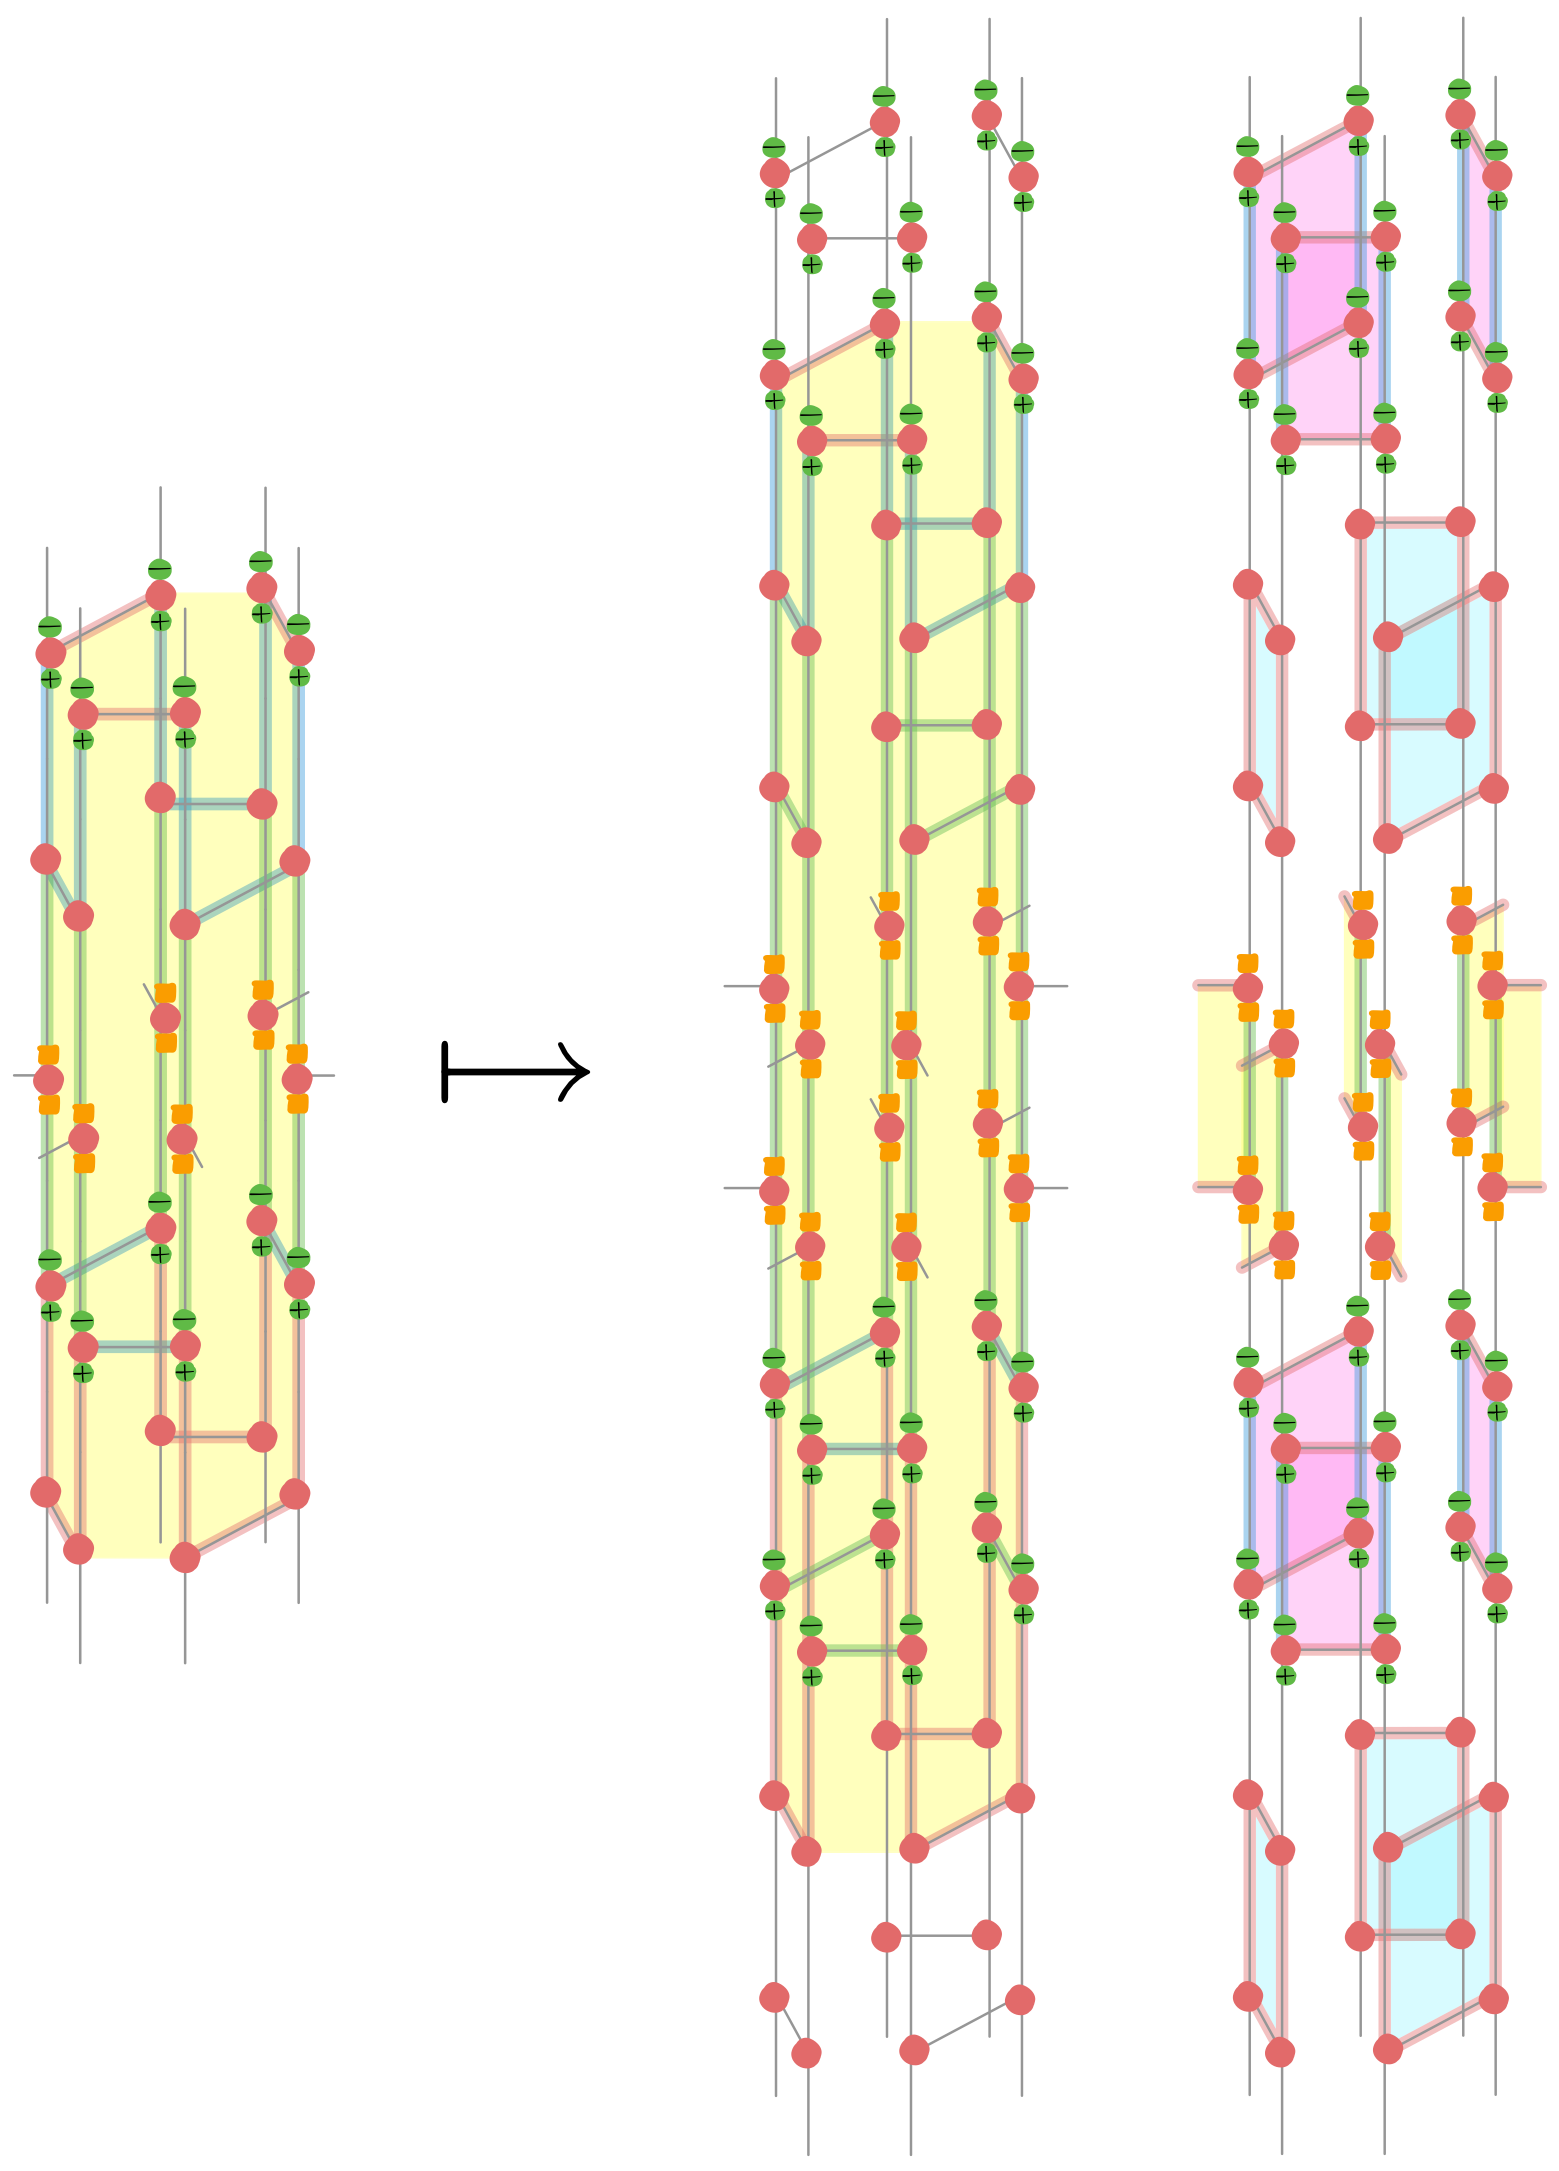
\includegraphics[width=0.6\linewidth]{figures/qubits/dcccs/repeating_measurements/detector_if_measurements_done_twice}
    \caption{Left: a detector in the $X^1 Y^1 Z^1$ code, involving 6 qubits, spanning 4 timesteps, and consisting of 12 measurements.Middle: the analogous detector in the repeated $X^2 Y^2 Z^2$ code, which still involves 6 qubits and 12 measurements, but now spans $(4-1) \cdot 2 + 1$ timesteps. Right: the edge detectors on these six qubits in the $X^2 Y^2 Z^2$ code, each of which spans one timestep and consists of two consecutive edge measurements.}
    \label{fig:detector_if_measurements_done_twice}
\end{figure}

Suppose we want to implement a DCCC on some physical hardware, but this hardware's noise is biased either towards a particular type of Pauli error (say, $Z$) or towards measurement errors.
An obvious thing we can do is think carefully about which DCCC to choose, because there are a number of differences between them that would affect performance under different noise models.

For example, detectors in the $X^1 Y^1 Z^1$ code consist of 12 measurements, while detectors in the $X^1 Z^1$ code consist of 6 measurements.
The intuition is that the fewer measurements involved in a detector, the better.
This is because the more measurements that are involved, the more likely the detector is to be violated,
and more violated detectors means more marked vertices in the decoding graph,
which makes the job of the decoder harder\footnote{A more accurate metric capturing this intuition is that of \textit{detector likelihood} \cite{hesner2024using}. This is the total probability of a set of errors occurring that violate a given detector. In the comparison between the $X^1 Y^1 Z^1$ and $X^1 Z^1$ codes, measurement errors are the only errors that contribute differently to the detector likelihood -- all data qubit errors affect the detector likelihood in the same way across the two codes.}.
So this difference between the two codes would suggest the $X^1 Z^1$ code might generally perform better, especially for measurement-biased noise.

Alternatively, another option available to dynamic stabilizer codes is to repeat certain measurements a number of times before moving to the next measurement in the operation schedule.
Static stabilizer codes don't have this freedom -- to implement a static stabilizer code, one simply measures the same set of Paulis indefinitely.
So we define the more general \textit{$X^aY^bZ^c$ honeycomb code} and the \textit{$X^aZ^b$ honeycomb code}, in which each round of measurements are repeated $a$, $b$ or $c$ times respectively.
In general, we call these \textit{repeated DCCCs} (so unrepeated DCCCs are a trivial subset of repeated DCCCs.)

The intuition here is that if our noise model is biased towards $Z$ errors, say, then we can spend more rounds repeatedly measuring $\dcccOp{e}{\kappa}{X}$ and $\dcccOp{e}{\kappa}{Y}$ edge operators, since consecutive such measurements will form detectors capable of detecting $Z$ errors.
We call these detectors \textit{edge detectors}, since each one can be associated with a unique edge, and call the other type of detectors \textit{face detectors}, since each one can be associated with a unique face.
Similarly, if our noise is biased towards measurement errors, the intuition is that repeating measurements increases the number of edge detectors, which consist of just two measurements.
These are therefore less likely to be violated by measurement errors, which should improve performance, as described in the second paragraph above.

These are the key ideas behind experimenting with repeated measurements, but in fact these two choices (choosing a different unrepeated operation schedule and then varying the number of rounds for which each set of measurements is repeated) have an array of effects on the resulting code, some in contrast with one another.
In the paper this section is based on, we investigated and explained these in a fair bit of detail.
The net effect, however, was not so dramatic -- different features cancelled one another out, and in the realistic but rather messy setting of circuit-level noise it gets hard to untangle exactly which effect causes which behaviour overall.
So rather than go into all the gory details, we content ourselves with having given the main intuition and move on to the numerical results.

\subsection{Numerical results}

We show four plots that summarise the performances of various repeated and unrepeated DCCCs under biased noise models.
The metric we use throughout is \textit{teraquop volume}.
Essentially, for a family of codes/circuits whose $j$-th member is defined on $n_j$ qubits and runs for an amount of time $T_j$, the teraquop volume is the smallest volume $n_j T_j$ such that the probability of any logical error occurring is $10^{-12}$.
So a smaller volume is better.
This is the natural generalisation of the teraquop footprint from a `space-only' picture to a `space-time' picture.

The key points revealed by \Cref{fig:phenomenological_noise_volume_plot_beliefmatching,fig:phenomenological_noise_volume_plot_pymatching}, which assume phenomenological noise, are that belief matching is a better decoder for the $X^a Y^b Z^c$ code while MWPM is a better decoder for the $X^a Z^b$ code, and that repeating measurements is in general effective against measurement-biased noise.

When we switch to circuit-level noise in \Cref{fig:pymatching_circuit_level_noise_volume_plot,fig:beliefmatching_circuit_level_noise_volume_plot}, we can still see that belief matching is a better decoder for the $X^a Y^b Z^c$ code while MWPM is a better decoder for the $X^a Z^b$ code.
However, repeating measurements is only worthwhile in a few specific cases.

\begin{figure}[p]
    \centering
    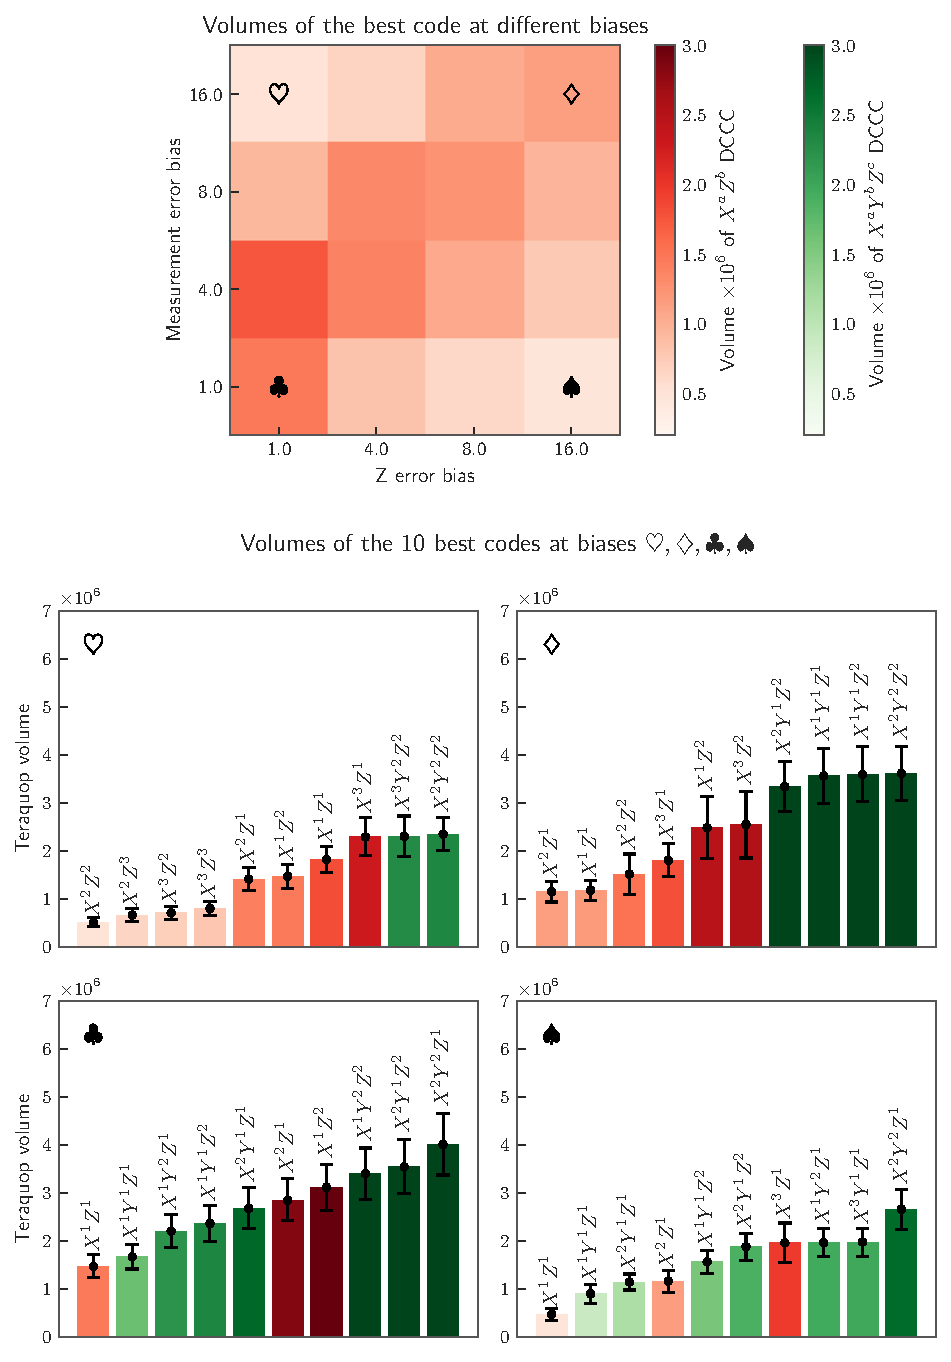
\includegraphics[width=0.9\columnwidth]{figures/qubits/dcccs/introduction/spacetime_volume_heatmap_pymatching}
    \caption{Squares in the top patchwork plot are red (green) if the code with the smallest teraquop volume is an $X^aZ^b$ code ($X^aZ^bY^c$ code).
    A darker shade indicates a higher volume.
    The four bar plots show the footprints of the 10 best codes at the four limits of the simulated biases.
    Decoding is performed using MWPM.
    For all noise models investigated here, the $X^a Z^b$ code outperforms the $X^a Y^b Z^c$ code.
    Repeating measurements improves performance when the noise is biased strongly towards measurement errors only, and has negligible effect otherwise.}
    \label{fig:phenomenological_noise_volume_plot_pymatching}
\end{figure}


\begin{figure}[p]
    \centering
    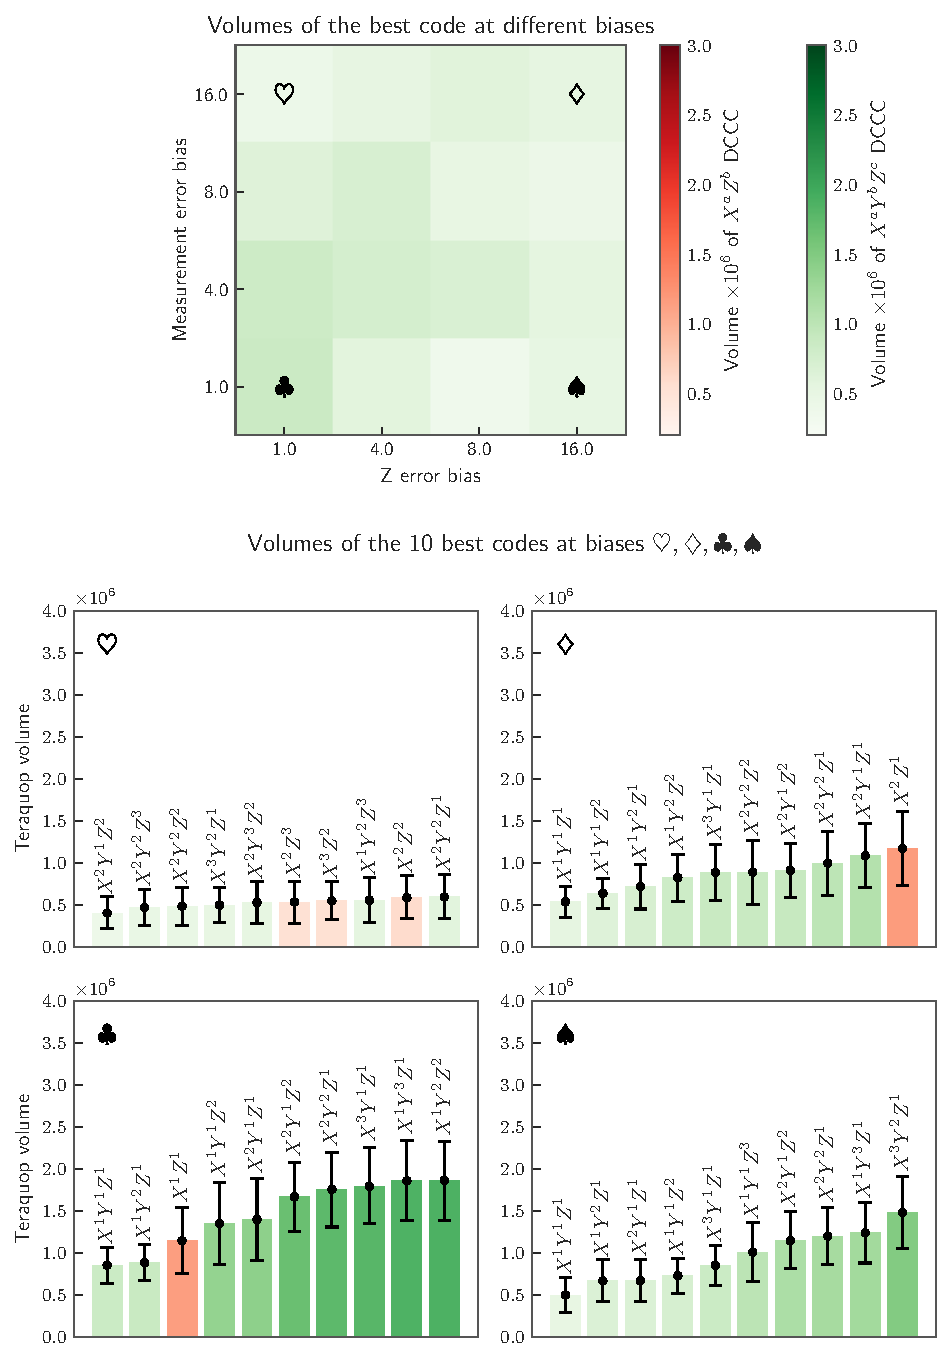
\includegraphics[width=0.9\columnwidth]{figures/qubits/dcccs/introduction/spacetime_volume_heatmap_beliefmatching}
    \caption{
        Same plot as in \Cref{fig:phenomenological_noise_volume_plot_pymatching} but with decoding performed using belief matching.
        In contrast to \Cref{fig:phenomenological_noise_volume_plot_pymatching}, for all noise models investigated here, the $X^a Y^b Z^c$ code outperforms the $X^a Z^b$ code.
        However, as before, repeating measurements improves performance when the noise is biased strongly towards measurement errors only, but has negligible effect otherwise.}
    \label{fig:phenomenological_issing_beliefmatching}
\end{figure}

\begin{figure}[p]
    \centering
    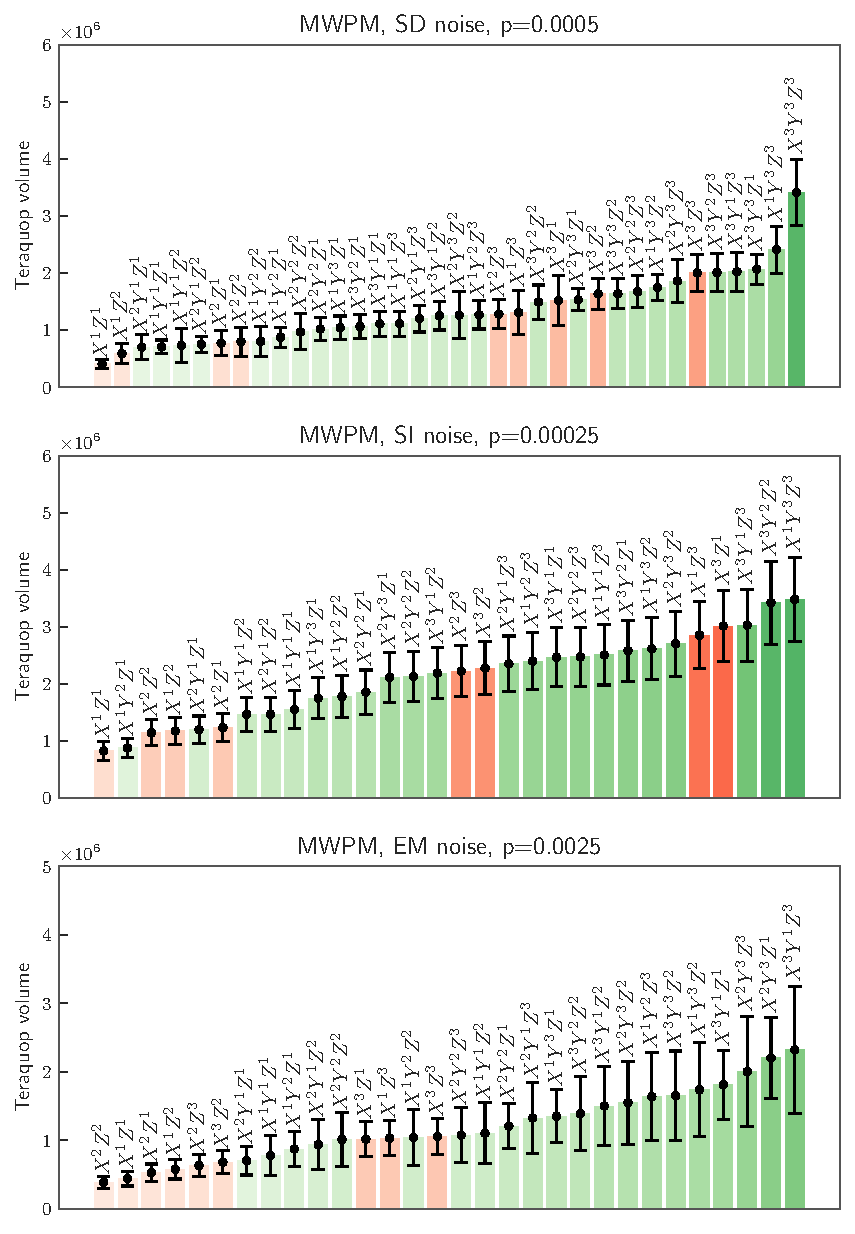
\includegraphics[width=0.9\columnwidth]{figures/qubits/dcccs/introduction/volumes_cln_pymatching}
    \caption{Teraquop volumes of $X^a Y^b Z^c$ and $X^a Z^b$ codes for three circuit-level noise models; standard depolarizing noise with $p=0.0005$, superconducting inspired noise with $p=0.00025$, and entangling measurement noise with $p=0.0025$. Decoding is performed using MWPM. In each case, the code with the best teraquop volume is from the $X^a Z^b$ family, though the difference
    is small.
    Repeating measurements broadly has negligible effect, though does seem to improve the performance of the $X^1 Y^1 Z^1$ code in the superconducting-inspired noise model, which features a moderate measurement bias.}
    \label{fig:pymatching_circuit_level_noise_volume_plot}
\end{figure}

\begin{figure}[p]
    \centering
    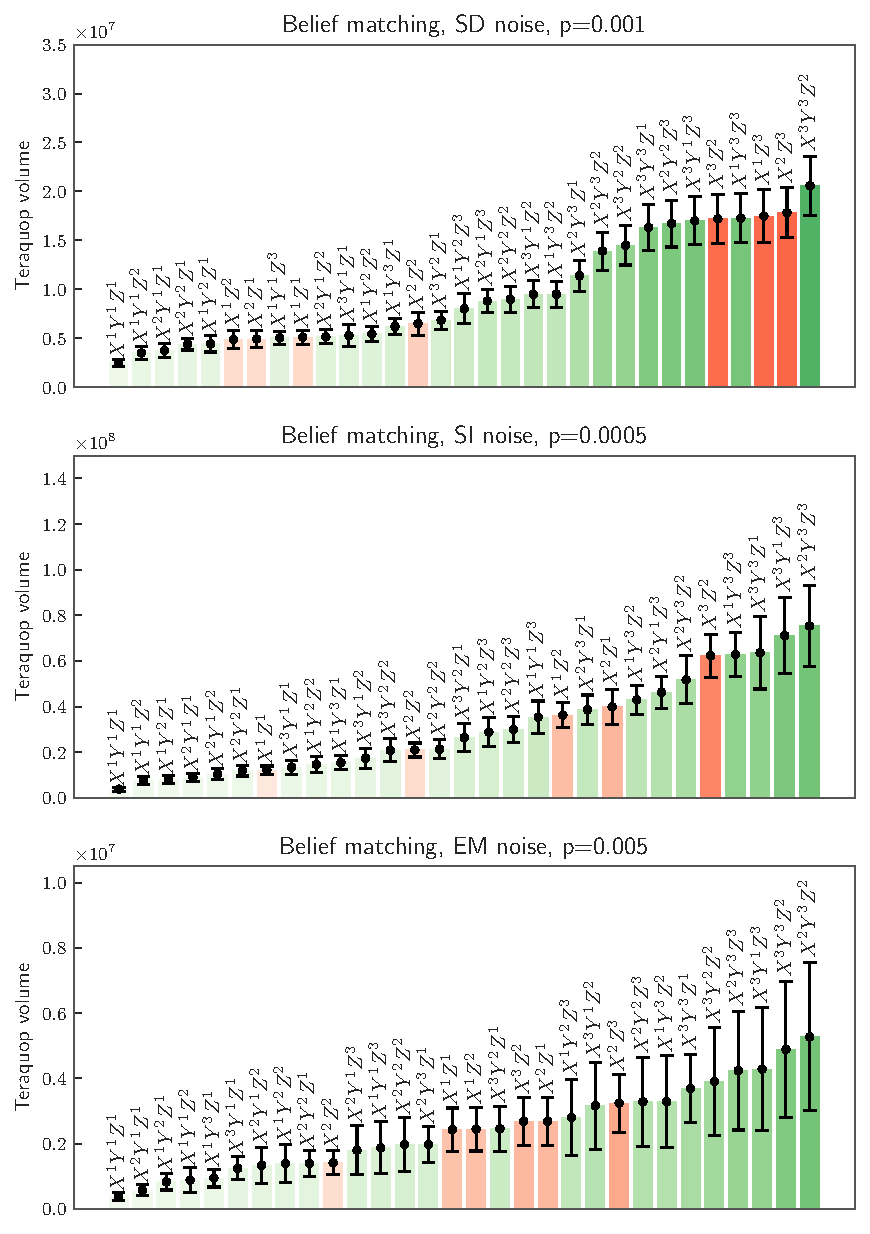
\includegraphics[width=0.9\columnwidth]{figures/qubits/dcccs/introduction/volumes_cln_beliefmatching}
    \caption{Teraquop volumes of $X^a Y^b Z^c$ and $X^a Z^b$ codes for three circuit-level noise models; standard depolarizing noise with $p=0.001$, superconducting inspired noise with $p=0.0005$, and entangling measurement noise with $p=0.005$. Decoding is performed using belief matching.
    In contrast to \Cref{fig:pymatching_circuit_level_noise_volume_plot}, now in each case the code with the best teraquop volume is from the $X^a Y^b Z^c$ family.
    As before, repeating measurements broadly has negligible effect, though does improve the performance of the $X^1 Z^1$ code in the entangling measurements noise model.}
    \label{fig:beliefmatching_circuit_level_noise_volume_plot}
\end{figure}
